\documentclass[12pt, letterpaper]{article}

% Language setting
% Replace `english' with e.g. `spanish' to change the document language
\usepackage[english]{babel}

% Set page size and margins
% Replace `letterpaper' with`a4paper' for UK/EU standard size
\usepackage[letterpaper,top=2cm,bottom=2cm,left=3cm,right=3cm,marginparwidth=2cm]{geometry}

% Useful packages
\usepackage{amsmath}
\usepackage{graphicx}
\usepackage[colorlinks=true, allcolors=blue]{hyperref}

\title{Image Classification of Monkeys}
\author{Mingjing Yin, Katie Li, Siyuan Liu}

\begin{document}
\maketitle


\section{Introduction}
 \quad \quad We are interested in whether photos of monkeys in ten different species taken with different postures and angles can be classified using existing classifiers. Also, we are interested in the ability of different classifiers to differentiate core differences that exist within portrait photos. Therefore, we propose our research question as---Which classifier can better classify monkey portraits? Specifically, which of the two classifiers can generate a better precision/recall score(accuracy score) when they are used to differentiate monkey species by their portraits.- One Versus One(OvO) method or Convolutional Neural Networks (CNN)? The following text will thoroughly explain the background of our data and method(OvO and CNN), the result and comparison of each method, the significance of our finding, and speculation for future research.


\section{Background of Data and Method}

\subsection{Data}

         \quad \quad We obtained our dataset from Kaggle. The dataset consists of two folders, a training set folder and a validation set folder. Each folder contains 10 sub folders labeled as n0~n9, each corresponding to a monkey species from Wikipedia's monkey cladogram. Images are 400x300 px or larger in JPEG format (almost 1400 images). Label mapping of our dataset is as follows:
         
         \bigskip
       
     n0: alouattapalliata, n1: erythrocebuspatas,
 
    n2: cacajaocalvus, n3: macacafuscata,
 
    n4: cebuellapygmea, n5: cebuscapucinus,
 
    n6: micoargentatus, n7: saimirisciureus,
    
    n8: aotusnigriceps, n9: trachypithecusjohnii.

        \bigskip
        Since our obtained data are tidy and well-categorized into training set and validation set, we first resize the image and directly standardize the image data to [0,1] when we conduct data preprocessing.

\subsection{Method}
       \quad \quad This project employs two image classification methods-- One Versus One (OvO) and Convolutional Neural Network(CNN) in TensorFlow, respectively. Convolutional Neural Network, one of the most famous image classification models for the classification of images in Deep Learning, has shown remarkable results in image classification(Setala, 2019). Discussion on CNN has touched on the application of CNN for document image classification(Kang et al., 2014), the implementation of CNN on multi-label image classification with images containing different objects, scenes, actions, and attributes(Wang et al, 2016), and CNN classification on hyperspectral image classification(Lee, Kwon, 2017). Convolutional Neural networks have been used for image classification in different fields widely. For example, in the medical field, Deep Convolutional Neural network-based medical image classification has been used broadly for disease diagnosis(Yadav et al., 2019) and Bacteria classification(Treebupachatsakul et al, 2019). Given both incredible results and the widespread uses of CNN in image classification, we chose CNN as our first choice for classifying photos of monkeys.
       
                      
        \begin{figure}
        \centering
        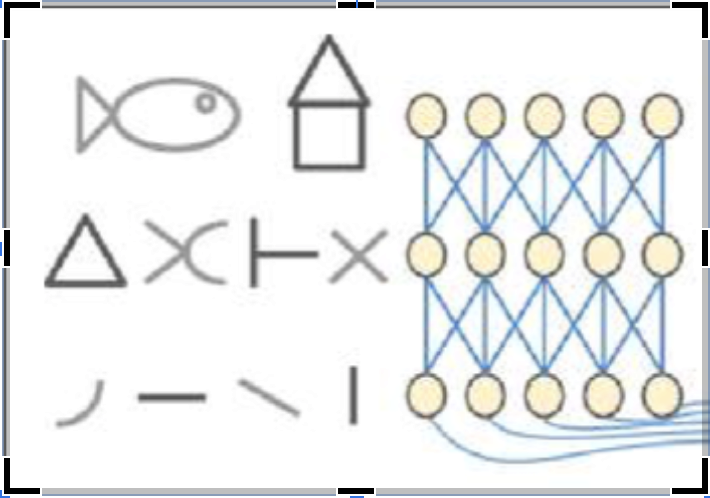
\includegraphics[width=0.5\textwidth]{image3.png}
        \caption{\label{fig:image3}Human visual neural network. From horizontal lines to triangular shapes, and to house-like objects(Olivas et al., 2009).}
        \end{figure}   
        
      The concept of the CNN classifier emerged from the study of the human visual cortex. An ordinary human has approximately 10 billion neurons in the visual cortex. Each neuron reacts to a small, local receptive field of the world we pierced. This receptive field can overlap, and combine into a much larger mental representation of the world. Neurons are also orientations and feature-specific. One neuron only reacts to a specific type of feature, like horizontal lines or curves. Higher-level neurons combine features returned from the lower-level neurons into more complex features as displayed in figure 1.
       
 
 
        Regarding One versus One(OvO) classifiers, we employed multinomial logistic regression algorithms of machine learning given the simplicity of this model. More recent attention has focused on Extreme Sparse Multinomial Logistic Regression for hyperspectral image classification(Cao et al., 2017). Current research has also demonstrated that the multi-class logistic regression method is superior compared to other conventional methods, especially when dealing with complex images(Ahmed et al., 2020). Thus, for monkey-species image classification, we employed both multinomial logistic regression and Convolutional Neural network methods to compare the accuracy level of these two methods.
 
\section{Result}

        \quad \quad For the OvO methods, the accuracy score on our testing data turns out to be 52.58 percent, which means that the percentage of correct prediction in the total number of data points is 52.58 percent. For CNN methods, we first train our model to an accuracy level up to 95.42 percent, which refers to the fact that the percentage of correct prediction in the total number of data points is 95.42 percent in the training set. Then, we evaluate the accuracy level of our testing data, which turns out to be 71.85 percent. This indicates that the percentage of correct prediction in the total number of the testing dataset is 71.85 percent. Based on the fact that 71.85 percent is significantly higher than 58.52 percent, we can conclude that the CNN model has a better performance in classifying the 10 species monkey dataset.

       After that, we make predictions using the CNN model and visualize the validating results using matplotlib. The visualizations are as follows:
       As shown in image 1, which refers to the first image that is predicted, the left part represents the prediction image and the right part represents the percentage of labels that are predicted as correct or incorrect. Specifically, the red column represents the wrong predictions and the blue column represents the correct predictions. As shown in image 2, which refers to the 12th image that is predicted using the CNN model, 93 percent of the images are predicted correctly. This can also be shown in the right part of the image in the blue column.
    \bigskip
      \begin{figure}[!ht]
       \centering
      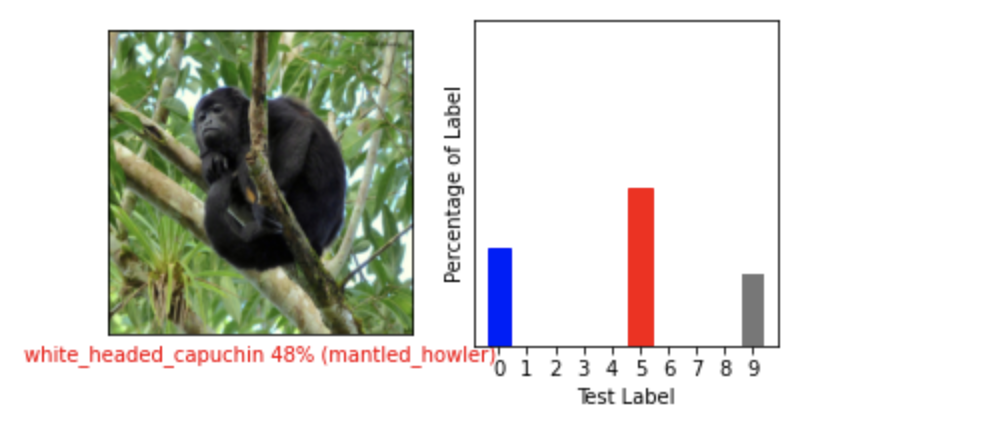
\includegraphics[width=0.8\textwidth]{image1.png}
      \caption{\label{fig:image 1}Image 1}
      \end{figure} 
      
      \begin{figure}[!ht]
       \centering
      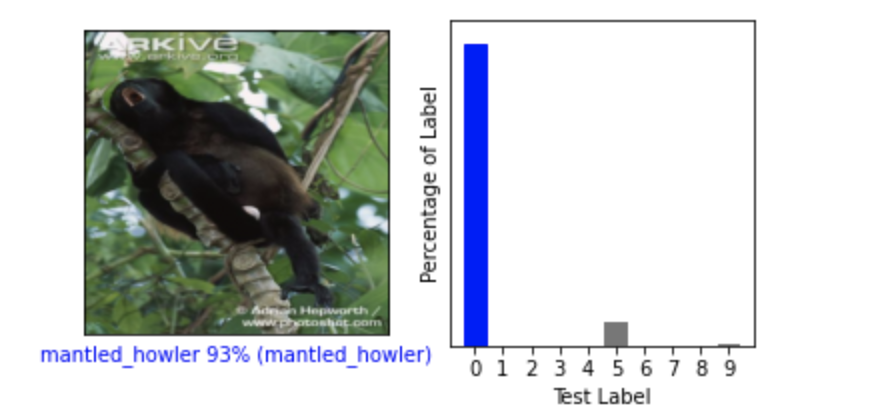
\includegraphics[width=0.8\textwidth]{image2.png}
      \caption{\label{fig:image 2}Image 2}
      \end{figure} 
    \bigskip
 
\section{Discussion }

        \quad\quad If the returned accuracy of one classifier is significantly different from the returned accuracy of the other classifier, we could conclude that one classifier has better performance in classifying the 10 species monkey dataset. Possibly, it could be generalized to other photo-based animal portrait datasets. In the current study, we again demonstrated that the CNN classifier is a more superior classification method compared to the normal logistic regression model(OvO). By using a filter to identify features, our classifier becomes less vulnerable and more adaptive to change in the monkey’s posture, angle, and size. So based on our codes presented previously, it is safe to say that CNN shows an overpowering advantage when it comes to differentiating photos. Due to small fluctuations in the accuracy score every time we run the code, the numbers 0.58 and 0.71 are simply estimations, but even then the difference is still big enough to observe an obvious advantage siding the CNN model. 
        
        There were multiple speculations on why CNN showed a better performance. Since we attempted to eliminate the result of overfitting by increasing our training set through rotating and zooming in on existing training photos, we concluded that the reason behind CNN’s performance it’s caused by the fact that while OvO compares picture as a whole, CNN is more observant of patterns that exist between monkeys of the same species. As you can see in Image 1, CNN will determine the similarities of patterns that exist between the image being classified and other determined images. This way, CNN is less likely to be distracted by outliers than the OvO model. In Image 1, while CNN determines that the image is 48 percent similar to other white headed capuchin monkeys, it also demonstrated that outliers are less likely to determine the outcome of the image due to the complex calculation that takes place. Having an outlier or two will not heavily influence the percentage of similarities. 
        
        When you compare Image 1 and Image 2, it is hard for the human eye to tell the differences between these two monkeys, so this is the main advantage of utilizing a CNN model for classification. CNN’s detected patterns are often so small and so trivial that we would’ve had a very hard time noticing that’s if we noticed the difference at all. In addition, even though the monkeys' position is wildly different between these two photos, CNN’s performance was not detrimentally affected. This is because CNN does not rely on positions and identifying features. The patterns detected are calculated by CNN’s algorithm and not guided by external influences. 
        
        If our conclusion is correct, then the application of our findings can be utilized in multiple different fields. Due to the pattern detecting nature of CNN, we believe that it can be used for emotion differentiation in humans, facial recognition, and speciation of other animals. The reason behind the use of CNN in emotion differentiation in humans is that while people of different cultures express emotion differently, they tend to utilize the same set of facial muscles when it comes to automatic responses such as laughter and disgust. CNN’s pattern detection can be trained to detect a set of muscle movements and allow it to classify them as different emotions. The use of CNN in facial recognition and speciation of other animals is similar to what we did today, the only challenge being that facial recognition requires the model to be more specific in the detection of the underlying pattern. Nevertheless, we believe that CNN has great potential and our use of CNN has been exceptionally educational.


       
 
\section{Contribution}

    
         Mingjing Yin: Writing Introduction, data, literature review, and results part of this report; Writing Codes; 5 minutes presentation explaining the codes; Github construction.
  
    Katie Li: Writing Discussion part of the report; 5 minutes presentation about discussion and implication; video editing.

    Siyuan Liu: Writing Methods part of this report; 5 minutes presentation explaining CNN; modifying format of Latex.
    
\section{References}
\medskip
Ahmed, A., Jalal, A.,  Kim, K. (2020). A novel statistical method for scene classification based on multi-object categorization and logistic regression. Sensors, 20(14), 3871.
\medskip
Cao, F., Yang, Z., Ren, J., Ling, W. K., Zhao, H.,  Marshall, S. (2017). Extreme sparse multinomial logistic regression: A fast and robust framework for hyperspectral image classification. Remote Sensing, 9(12), 1255.
\medskip
Kang, L., Kumar, J., Ye, P., Li, Y., Doermann, D. (2014, August). Convolutional neural networks for document image classification. In 2014 22nd International Conference on Pattern Recognition (pp. 3168-3172). IEEE.
\medskip
Lee, H.,  Kwon, H. (2017). Going deeper with contextual CNN for hyperspectral image classification. IEEE Transactions on Image Processin
\medskip
 Olivas, E. S., Guerrero, J. D. M., Martinez-Sober, M., Magdalena-Benedito, J. R.,  Serrano, L. (Eds.). (2009). Handbook of research on machine learning applications and trends: Algorithms, methods, and techniques: Algorithms, methods, and techniques. IGI Global.
 \medskip
Treebupachatsakul, T., Poomrittigul, S. (2019, June). Bacteria classification using image processing and deep learning. In 2019 34th International Technical Conference on Circuits/Systems, Computers and Communications (ITC-CSCC) (pp. 1-3). IEEE.


\medskip
Wang, J., Yang, Y., Mao, J., Huang, Z., Huang, C.,  Xu, W. (2016). Cnn-rnn: A unified framework for multi-label image classification. In Proceedings of the IEEE conference on computer vision and pattern recognition (pp. 2285-2294).
\medskip
Yadav, S. S., Jadhav, S. M. (2019). Deep convolutional neural network based medical image classification for disease diagnosis. Journal of Big Data, 6(1), 1-18.


\end{document}

